\documentclass[10pt,conference]{IEEEtran}
\IEEEoverridecommandlockouts
% The preceding line is only needed to identify funding in the first footnote. If that is unneeded, please comment it out.

\usepackage{cite}
%\usepackage{fontspec}
\usepackage{amsmath,amssymb,amsfonts}
\usepackage{algorithm}
\usepackage{algorithmicx}
\usepackage{fullwidth}
\usepackage{algpseudocode}
\usepackage{graphicx}
\usepackage{subfigure}
\usepackage{textcomp}
\usepackage{xcolor}
\usepackage{listings}
\usepackage{multirow}
\def\BibTeX{{\rm B\kern-.05em{\sc i\kern-.025em b}\kern-.08em
T\kern-.1667em\lower.7ex\hbox{E}\kern-.125emX}}
\begin{document}
\author{
\IEEEauthorblockN{Qian Li, Jiao Zhang, Tao Huang, Yunjie Liu}
\IEEEauthorblockA{State Key Laboratory of Networking and Switching Technology, BUPT, China
\\Email: \{liqian06, jiaozhang, htao, liuyj\}@bupt.edu.cn}
}

\title{Data-driven Routing Optimization based on Programmable Data Plane}
%{\footnotesize \textsuperscript{*}Note: Sub-titles are not captured in Xplore and
%should not be used}
%\thanks{Identify applicable funding agency here. If none, delete this.}
%}

\maketitle

\begin{abstract}
To meet the growing demand for high bandwidth of Multimedia network, IP Network Providers spend millions of dollars overprovisioning bandwidth of their network. However, due to the lack of reasonable traffic scheduling, the over-provisioning network still has a severe issue of utilization imbalance. Traffic Engineering (TE) is proposed to solve this problem. Network measurement and routing optimization strategies are two key components of TE. Existing out-band network telemetry that transmits extra probes to measure network status has the problem of inaccurate measurement information in the highly time-varying network. And the relationship between complex network status and routing optimization strategy is difficult to describe with an exact mathematical model. Therefore, we propose a novel TE approach, which is called DPRO. It combines In-band Network Telemetry based on programmable language P4 with Reinforcement Learning to minimize network congestion. Extensive experiments show that our approach significantly outperforms several widely-used baseline methods in terms of max-link-utilization.
\end{abstract}
%which greatly affects the reliability and availability of the network, Effective real-time network measurement provides the basis for the generation of route optimization strategy, which makes the network congestion-aware.
\begin{IEEEkeywords}
Traffic Engineering, P4, Reinforcement Learning, In-band Network Telemetry
\end{IEEEkeywords}

\section{Introduction}
%problem statement, why TE is so important, the challenges, current solutions, new ideas, performance summary, main contributions of the paper(optional), structure of the paper. 1/2 page.
%demand, low utilization, TE is needed and important. TE challenge.
The Internet has currently changed into a Multimedia network, which supports many types of multimedia applications with high bandwidth demand. Thanks to the rapid development of communication network hardware, IP network providers can adopt a strategy of bandwidth overprovisioning in their networks to support the sharply growing traffic of customers\cite{TE-survey2008}. However, this approach is no longer applicable due to the increasing traffic demand, the high update cost, and the low link utilization. Traffic Engineering (TE) is proposed to solve this problem.
%As stated by the Internet Engineering Task Force (IETF), TE deals with the performance optimization of operational networks and plays a key role in the provisioning of services with Quality of Service (QoS)\cite{Awduche1999}.

%Simple and widely-used TE solutions include always routing traffic via shortest paths (e.g., Open Shortest Path First (OSPF)); or evenly distributing traffic via multiple available equal-cost paths (e.g., Equal Cost Multi-Path (ECMP)). Neither of them is optimal because they are network unawareness and are easy to cause network congestion with the burst traffic coming. Some SDN-based related works \cite{Fortz2002}\cite{Sridharan2005}\cite{Fortz2000}\cite{Fortz2002a} aim to manage flow traffics by requiring timely detection of significant flows that carry a large amount of data or important paths. And optimize the OSPF by sending probes to measure network status and combining some greedy algorithms to calculate traffic distribution. But there are two shortages in these methods: 1) The results of probe measurements are not accurate because the network is highly time-varying. The network state when the node receives the probe is often different from the network state when the probe is in flight. 2) The relationship between network state and routing optimization strategy is difficult to express with an accurate mathematical model. Besides, too complex mathematical models often place high demands on network nodes that run the models.
%
%The goal of traffic engineering is to optimize routes based on network state. Therefore, there are two key challenges: how to monitor network status with the granularity as fine as we can and how to transform the network status into proper routing optimization strategies as accurate as we can. The development of emerging technologies, Software-defined Networking (SDN)\cite{mckeown2009software}, has presented us with new ideas for solving TE. Flexible and programmable data plane makes the network more operational and transparent. We can get the real network state when the packet is processed by In-band Network Telemetry (INT) \cite{kim2015band} using the domain-specific language P4\cite{p42014}. The recent breakthrough of Reinforcement Learning (RL)\cite{kaelbling1996reinforcement} provides a promising technique for enabling effective experience-driven model-free control, which hit us that we can combine RL into a centralized control plane to make decisions. The control plane in logic central acts as the brain of the network to collect network information, decision-making and deployment solutions.
%Simple and widely-used TE solutions either route the traffic to shortest paths (e.g., Open Shortest Path First (OSPF)) or evenly distribute it to multiple available equal-cost paths (e.g., Equal Cost Multi-Path (ECMP)). Neither of them is optimal because they are network-unaware and are easy to cause network congestion with the burst traffic coming.
Network measurement and routing optimization strategies are two key components of traffic engineering (TE). Correspondingly, there are two major challenges to designing a good TE solution. One is that the current network measurement can not report network status accurately and timely. Some related works \cite{alizadeh2014conga}\cite{akyildiz2014roadmap}\cite{katta2016hula} aim to manage flow traffic by timely detection of significant flows or links that carry a large amount of data, with existing out-band network telemetry (ONT) methods. For example, NetFlow \cite{estan2004building} tries to detect network status by periodic polling of traffic statistics from switches, and \cite{wang2004sflow} achieves network measurement by sampling packets from switches. However, these ONT methods have high monitoring overheads, which easily incur significant switch resource consumption and long detection times. Another key challenge of TE is that the relationship between network state and routing optimization strategy is quite difficult to describe with an exact mathematical model\cite{Azar2003Optimal}. Besides, overly complex mathematical models often place high demands on the storage and computing resources of the network nodes that run the model.

The development of Software Defined Networking (SDN)\cite{mckeown2009software}, has presented us with new chances for TE. Flexible and programmable data plane makes the network more operational and transparent. The novel network measurement, INT (In-band Network Telemetry) \cite{kim2015band}, allows the cost-effective network monitoring by encapsulating device-internal states into probe packets. With INT, we can get the real-time network status information with the finest granularity we desire, and that is the basis of good routing optimization strategies. Also, the recent breakthrough of reinforcement learning (RL)\cite{kaelbling1996reinforcement} provides a promising technique to enable effective experience-driven model-free control. It hits us that we could combine RL with a centralized control plane to make decisions.
%Some related works \cite{DRL-TE}\cite{learning-to-route} attempts to use reinforcement learning for routing optimization by exploiting the continuous interaction of agent and environment to learn a non-linear mapping relationship, which seems to be a promising direction for TE.

Therefore, we propose an innovative and highly effective data-driven, model-free TE solution called DPRO in this paper. In DPRO, the data plane is responsible for timely monitoring network states with INT. Based on the network status uploaded by the data plane, the control plane performs route optimization under the guidance of a reinforcement learning algorithm.

On the flip side, leveraging INT information and reinforcement learning in TE is not straightforward. There are two main challenges to design DPRO. First, the P4-based INT specification\cite{kim2015band} defines a reference format for packet encapsulation, including all metadata that INT can measure within the device. However, this encapsulation format in \cite{kim2015band} takes up a lot of processing latency for the switch, and not all information is what DPRO needs. Therefore, we redesign the P4-based packet processing logic to combine INT with the processing of regular packets in DPRO. Second, the design of the model has a lot to do with performance in reinforcement learning. If the correlation between input and output in the reinforcement learning model is small, the RL model may be difficult to converge to satisfactory performance. Our approach simplifies the complexity of the reinforcement learning model by learning the mapping from link loads to link weights, speeding up the model's convergence.
%The control plane in logic central acts as the brain of the network to collect network information, make decisions and deploy solutions.
%We can get the real-time network state when the packet is processed by In-band Network Telemetry (INT) \cite{kim2015band} using the domain-specific language P4 \cite{p42014}.
We summarize our contributions in the following:
\begin{itemize}
\item We are the first to propose a complete practical INT-based data-driven control framework, DPRO, for TE.
\item We design a clever switch packet processing logic based on programmable language P4 to enable fast forwarding and ultra-low overhead measurement.
\item We show via building an experimental platform that DPRO significantly outperforms several widely-used baseline methods concerning three metrics, including max-link-utilization, flow completion time and packet delay.
\end{itemize}

%We organize the remaining of this paper as follows. Section II presents the main concepts and technologies that influenced our thinking, then, we show our motivation. Section III describes the design details of DPRO. Section IV presents the evaluation results of DPRO. Finally, Section V concludes the paper.
\section{Background and Motivation}
%a brief intro. of P4 and INT models used assumptions made
% P4 and INT 强化学习模型 问题定义。
In this section, we present the background that is necessary to understand the main aspects of our approach, with a focus on the programmable data plane and reinforcement learning. Then, we discuss some prior works and our motivation.
\subsection{Background}\label{ppo}
% we detail our proposal to reach network measurement in real-time with low overhead and minimize congestion with the help of reinforcement learning.
%The logical centralized network control and management architecture in SDN greatly improves the state consistency and reliability of the network. At the same time, the additional challenges inherent in single-point failures in a centralized architecture are unquestionable. At present, the industry mainly relies on horizontally expanding backup controllers to reduce the impact of single-point failures.

%In the early stage of SDN development, the logically centralized controller interacts with switches in the data plane through the southbound interface defined by the OpenFlow protocol. The data plane forwards the data packet according to the rules delivered by the control plane. When the header field of a packet matches the rule in the flow tables successfully, the corresponding action (such as dropping or forwarding) of the entry is triggered. When the match fails, a default action of reporting to the controller or directly discarding the packet is taken.
%
%To meet the needs of network development, the number of matching fields that can be supported in OpenFlow continues to increase, which greatly reduces the flexibility of OpenFlow protocol and hinders the market promotion of OpenFlow hardware switches. Because the match fields of OpenFlow switch are solidified on the switch chip and the modification of the protocol indicates that the hardware switch needs to be redesigned to support the latest features.

\emph{1) Programmable data plane}: The emergency of data plane programmable language P4\cite{p42014} greatly solves the limitations imposed by the OpenFlow protocol. Unlike the OpenFlow protocol, P4 is a high-level language for programming protocol-independent packet processors, and it intends to be used for the description of package processing capabilities of programmable switches. Compared with OpenFlow which has fixed header fields, P4 can custom the header fields of the packet and the processing workflow. This new type of interaction with the forwarding devices can effectively bring programmability.

The P4 code is compiled specifically for a platform and requires the compiler to be compatible with the hardware architecture. An API is auto-generated and allows control plane to operate table rules or other objects.
% In this section, we provide a brief introduction to reinforcement learning.

\emph{2) Reinforcement learning}: In the reinforcement learning framework, an agent repeatedly interacts with an environment in discrete decision epochs. At the beginning of each time epoch $t$, the agent observes the current state $s_{t}$, of the environment and selects an action $a_{t}$ from a fixed set of actions. Once the agent makes a decision and chooses an action $a_{t}$, the state of environment changes into $s_{t+1}$, and the agent receives a reward $r_{t}$ that signifying how good or bad the action that the agent took was. Therefore, the agent needs to try and try gradually, learn the environment and adjust its own decisions to achieve a greater reward. Finally, the agent learns a mapping $\pi$ from the set of possible states $\widehat{S}$ to the space of actions $\widehat{A}$. A more detailed exposition of reinforcement learning can be found in \cite{kaelbling1996reinforcement}.
\subsection{Prior Work}
%Priori work including optimizing OSPF or IS-IS weights\cite{Fortz2002} and MPLS tunnels \cite{elwalid2001mate}\cite{kandula2005walking},optimizing for bulk data transfers using relay nodes \cite{laoutaris2011inter}. These studies focus on optimizing bandwidth allocation and disregard the possibility of failures.
\emph{1) Traffic management}: TE optimization is a well-researched challenge. Recent interest in centralized TE is driven by SDN to running and optimizing such networks at scale (such as B4\cite{jain2013b4}, FFC\cite{liu2014traffic}, and Teavar\cite{bogle2019teavar}). These schemes exploit a global view of the network and perform global updates to configure flow allocations.
%An accurate network measurement can help us understand what happened in the network box to manage the network more effectively.

\emph{2) Network measurement}: In-band network telemetry is a hot topic in recent years. \cite{pan2019int} proposes INT-path, a network-wide telemetry framework, by decoupling the system into a routing mechanism and a routing path generation policy, transforming network troubleshooting into pattern recognition problems. HPCC \cite{li2019hpcc} is a new high-speed congestion control mechanism, which leverages in-band network telemetry to obtain precise link load information and controls traffic precisely.
\subsection{Motivation}
In recent years, the outstanding performance of machine learning especially reinforcement learning in other fields (such as AlphaGo\cite{silver2016mastering}), attracts the attention of network researchers. More and more attempts have been made to exploit machine learning techniques to solve network problems, such as TE. \cite{learning-to-route} is the first attempt to introduce reinforcement learning to the TE problem. It takes the traffic matrix of $K$-long historical time slices as input and the weight of all links as the output to minimize network congestion. DRL-TE \cite{DRL-TE} presents an experience-based DRL-based control framework for TE and aims to learn the proportion of traffic distribution of $K$ TCP streams on multiple sub-paths.

These above studies all focus on the design of machine learning models, but the overall scalability and operability of these schemes are neglected. For example, \cite{learning-to-route} assumes that the flow demand matrix in each time slice is fixed and can be accurately calculated or well predicted by network measurement. But this assumption has always been a lot of controversy \cite{DRL-TE}. Otherwise, \cite{DRL-TE} has no consideration of scalability problems in the RL model. When the number of TCP connections in the network increases, the state space and action space of the reinforcement learning model will increase sharply. Until then, the learning rate and efficiency of the machine learning algorithm will decrease and the performance of DRL-TE will be difficult to guarantee.

Motivated by these approaches, we try to propose DPRO, a complete data-driven control framework for TE, based on fine-grained and real-time network measurement with INT. We describe the details of our approach in the following sections.

\section{Design}

DPRO addresses TE problems with the perspective of integration between the data plane and the control plane. Fine-grain network measurement in real-time is supported by the data plane, while route updates that require a global view of the network are performed by the control plane. As such, DPRO relies on an adaptive feedback control-loop: an offline control-loop that is periodically executed by the controller to analyze routes and make global changes, based on the network status uploaded by the data plane. An overview of DPRO is shown in Fig.\ref{design}.
%This hybrid routing optimization strategy relies on data and control plane programmability, using respectively the P4 language \cite{p42014} and a switch-compatible interface similar to what exists in OpenFlow to update rules. The separation between planes becomes clear and makes switches express high forwarding capacity and network measurement, leaving complex tasks such as decision-making to controllers with sufficient resources.
\begin{figure}[t]
\centerline{\includegraphics[width=3.5in]{pic/design.pdf}}
\caption{The overview of DPRO}
\label{design}
\end{figure}
\subsection{Design of Data Plane using P4}
In our proposal, we program the processing logic of switches with programmable language P4\cite{p42014} to implement both forwarding and monitoring tasks.

\emph{1) Data plane routing mechanism:} The flow concept is defined by the tuple: source IP, destination IP, protocol version (4 or 6), the source port, and the destination TCP port. Our proposal is routed at the granularity of flow. Routing optimization with flow granularity has many advantages over granularity with packets or Flowlet\cite{Kandula2007Flare}. To minimize the number of flow rules in the P4 switches and therefore, reduce the network reconfiguration time, we use a special flow header with the following format to guide forwarding:

%The routing optimization strategy based on packets needs to consider the rearrangement loss caused by the out-of-order problem. Routing optimization based on Flowlet requires consideration of the identification and partitioning of sub-flows. The basic principle of Flowlet is to divide a stream into segments of multiple consecutively arriving packet groups. It is divided into one or more sub-flows by monitoring the time interval at which each packet segment of a stream arrives. However, it should be noted that in different scenarios, the time interval as a segmentation standard is different, and it is difficult to have a uniform division.
\begin{lstlisting}[breaklines,columns=flexible,basicstyle=\footnotesize,language={C},tabsize=4,keywordstyle=\bfseries,stringstyle=\ttfamily,escapeinside=``,commentstyle=\color{red!50!green!50!blue!50},showstringspaces=false]
	`\textbf{header}` flow_header_t {
		count:8;	//number of hops
		routeid:16;	//identifier of the path
		protocol:8;	//1:sample flag, 0:no sample
	}
\end{lstlisting}

On the data plane, each switch can logically plays an intermediate or endpoint role. As for route tasks, all the decisions over the flows happen at the endpoints. The endpoint switch is responsible for switching flows between the routes installed by the controller as well as inserting the flow header (flow\_header). For the intermediate nodes, they only need to perform the forwarding operation between the input port and the output port, thereby reducing processing and memory usage. Thus, intermediate switches do not need to perform any flow header modification.

\emph{2) Data plane measurement mechanism:} Network measurement is a vital part of traffic engineering. Because the measurement results not only can provide feedback on the policy adjustments of the TE control subsystem but also can be an important tool for judging how good or bad the TE solution is. In this work, we try to use in-band network telemetry (INT) \cite{kim2015band} technology to measure network states through inflight packets, which is more accurate and reliable as well as wasting little bandwidth overhead. We discuss the overhead of network measurement with INT in Section \ref{results}.
%The latest works about traffic engineering such as \cite{learning-to-route} are based on the assumption that the traffic matrix can be accurately measured and evaluated, but this assumption is exactly where the most controversial aspects of these solutions are.

In-band network telemetry relies on the processing pipeline in the P4 switch. During the processing of a packet, P4 switch records all metadata information of the packet inside the switch, which contains queueing delay, input port, queue depth when leaving the queue and so on. Besides, a counter entity is used to record the forwarding bytes or packets of each port in the P4 switch. The statistics of the counter entity can directly be read or reset by the control plane through the counter interface at any time.

\emph{Based on the above features of P4 switches, we try to use INT based on P4 language to measure network status through inflight packets in DPRO, especially link load and switch node load. }The \emph{link load} is defined as the ratio between the amount of data being transmitted on the link in a sampling period and link capability. In DPRO, the centralized controller can read the counter statistics of ports at both ends of a link through the counter interface, thus, the load of the link in a period can be obtained after simple calculating. \emph{Switch node load} has never been considered as metrics of network states in prior TE solutions, but it is also a very important parameter to indicate the network status. In the theoretical model of the communication network, the node cost is often averaged to all edges separated from the node, which can illustrate that switch node cost should also be considered when selecting the best path. Due to the lack of a unified definition of node load, we define the ratio between the queue depth and the limited length of the queue as the switch node load in DPRO.

As for measuring tasks, we can program the processing logic of switches to achieve periodic automatic sampling of packets. And the INT information is piggybacked on inflight packets. Specifically, only the endpoints are responsible for setting sampling flag and all switches perform inserting INT information with a format as follows when meeting sampling flag:

\begin{lstlisting}[breaklines,columns=flexible,basicstyle=\footnotesize,language={C},tabsize=4,keywordstyle=\bfseries,stringstyle=\ttfamily,escapeinside=``,commentstyle=\color{red!50!green!50!blue!50},showstringspaces=false]
	`\textbf{header}` int_t {
		swid:8; //identifier of switch
		qdepth:16;	//the depth of queue when the packet was dequeued
	}
\end{lstlisting}

\emph{3) Packet processing logic:} When a new packet arrives at the edge switch, the packet header field will be parsed firstly in the defined order as depicted in Fig.\ref{parser}. P4 describes state machine that traverses packet headers from start to finish, directly as the set of transitions from one header to the next. Each transition may be triggered by values in the current. Here, we define that the \emph{etherType} field in the Ethernet header is 0x801, indicating that the next header type is the route header (flow\_header). The \emph{protocol} field of the routing header is 0x01, indicating that the next header type is the measurement header (int\_header). After the parser block, the extracted headers are forwarded to the control block for processing.
\begin{figure}[t]
\centerline{\includegraphics[width=3.5in]{pic/parser.png}}
\caption{Parser order}
\label{parser}
\end{figure}

The complete logic of a packet being processed in the control block is shown in Alg.\ref{data-process}. If the flow is new, the flow\_header should be added to all packets of the flow by applying \verb| create_flow_header| table. The \verb|create_flow_header| table is indexed by IP/mask and is used to store the active route identifiers grouped by source-destination node pairs. To avoid the ``herd'' mentality, $K$ equivalent paths are configured by the controllers between each pair of nodes. 
\begin{algorithm}
\caption{Data Plane Packet Processing}\label{data-process}
\begin{algorithmic}[1]
\Procedure{control ingress}{}
\If {$\text{meta.routeid} = \text{0}$}
\State \textbf{apply} \emph{create\_flow\_header}
\State \textbf{apply} \emph{check\_register}
\If {$(\text{current\_tstamp} - \text{last\_sample\_tstamp}) > T_s $}
\State \textbf{apply} \emph{set\_sample}
\EndIf
\EndIf
\State \textbf{apply} \emph{routeid\_fwd}
\If {$\text{eth.ethType} = \text{0x0800}$ \& $\text{flow\_hdr.pro} = \text{0x01}$}
\State \textbf{apply} \emph{clone\_to\_controller}
\EndIf
\EndProcedure
\State
\Procedure{control egress}{}
\If {$\text{flow\_hdr.pro} = \text{0x01}$}
\State \textbf{apply} \emph{add\_load\_info}
\EndIf
\If{$\text{std\_meta.istance\_type} = \text{0}$ \& $\text{eth.ethType} = \text{0x0800}$}
\State \textbf{apply} \emph{remove\_additional\_header}
\EndIf
\If{$\text{std\_meta.istance\_type} = \text{2}$}
\State \textbf{apply} \emph{update\_clone\_flag}
\EndIf
\EndProcedure
\end{algorithmic}
\end{algorithm}
According to the target IP, the flow matches one route group, then chooses an appropriate path number according to the result of the five-tuple hash. Besides, \verb|routeid_fwd| table is indexed by the route identifier and returns which port to be forwarded. As for sampling tasks, \verb|check_register| table and \verb|sample_flag| table are designed to set sample flag. Specifically, \emph{protocol} field in flow\_header is bound to be set to 1 when the time interval between the arrival of the current packet and the last sampling exceeds the sampling period $T_s$. \verb|add_load_info| table is a no index table and used to add INT information as listed in int\_t header to sampling packets.

When the packet arrives at the destination switch and is bound to be delivered to the target host next, the packet should be reverted to the normal format for reception by the destination host, that is, the flow\_header (that used to guide routing)and int\_header (that used to carry INT information) should be removed (\verb|remove_additional_header| is applied). Before that, the packet is bound to be replicated (\verb|clone_to_controller| is applied) if there is some load information carried on the packet header. Note that the processing of normal packets and replicated packets are independent of each other. The normal packet will be sent to target hosts while the replicated packet will be delivered to a special port that connects to the controller.

\subsection{Control Plane Operation}
In DPRO, the centralized controller is responsible for delivering route optimization strategies with a global view of network status. However, because the regularity of network state changes is difficult to figure out, we try to use reinforcement learning techniques with self-exploration characteristics to perceive network changes and thus, assist in the generation of route optimization strategies.

\emph{1) Design of reinforcement learning model}: To utilize the RL techniques (no matter which method/model to use), we first need to design the state space, action space, and reward function. Note that the design of state space, action space and reward is critical to the success of an RL method.
\begin{itemize}
\item\emph{State Space}: The state space consists of two components: link load and switch node load. Formally, the state vector is defined as $S$, where $l_i$ is the link load of link $i$ and $s_j$ is the node load of switch $j$.
\begin{equation*}
\begin{aligned}
S=(l_1, l_2,...,l_i,...,l_n,s_1,s_2,...,s_j,...,s_m)
\end{aligned}
\label{state}
\end{equation*}

\item\emph{Action Space}: Considering that the direct output routing strategy or traffic distribution ratio will make the action space too large, affecting the performance of the RL model, thus we decide to regard the weight values of all edges in the network as the action space. Formally, the action vector is defined as $A$, where $w_i$ is the weight value of link $i$ and $|w_i|<=2$.
\begin{equation*}
\begin{aligned}
A=(w_1,w_2,...,w_i,...,w_n)
\end{aligned}
\label{action}
\end{equation*}
\item\emph{Reward}: Minimizing congestion is the most basic optimization goal of TE. Because in an IP network, congestion can affect latency, jitter and even packet loss. Minimizing congestion can also indirectly reduce flow completion time and increase overall network throughput. Therefore, our optimization goal is to minimize congestion (a.k.a. minimize max-link-utilization). Formally, the reward is defined as $R$, where $u_i$ is the link utilization of link $i$.
\begin{equation*}
\begin{aligned}
R=-max(u_1,u_2,...,u_i,...u_n)
\end{aligned}
\label{reward}
\end{equation*}
\end{itemize}

In DPRO, time is divided into consecutive intervals, called ``epochs''. At the beginning of each epoch $t$, the controller (agent) decides on a routing strategy $R^{(t)}$ for that epoch based on the routing strategies and the network load status, which constitutes the observed state $S^{(t)}$ of the environment at that point. Then, the state changes as the network load status for epoch $t$, $S^{(t+1)}$, is revealed and the reward $R^{(t)}=-u(t)$ is received, where $u(t)$ is the max-link-utilization under $R^{(t)}$ for $S^{(t+1)}$. Our goal is to learn a mapping from network load status to the weights of links that maximize the expected discounted reward, as formulated above.

The TE problem is a continuous control problem. PPO algorithm is a state-of-the-art deep reinforcement learning algorithm PPO\cite{ppo2017} for continuous control and its basic idea has been introduced in Section \ref{ppo}. Thus, we choose PPO\cite{ppo2017} algorithm for our approach.

\emph{2) Routing update mechanism}: Based on the weights of network links which are the output of PPO algorithm, the Dijkstra algorithm is used to calculate the shortest path between all pairs of source-destination nodes. Then, the optimal path is bound to replace the current worse path between a pair of nodes. Traffic engineering is generally an online strategy, and the traffic status changes quite violently. However, the excessively large-scale adjustment of the network routing policy is likely to cause the instability of the route, inducing route oscillating and packet loss. To solve this problem, we use the polling method to update the routing entries of all pairs of nodes. That is, the routing policy of only one pair of source-destination nodes will be updated within an update period $T_u$.

%And this issue may greatly reduce the Quality of Service (QoS) and user experience for some high-quality requirement applications such as audio and video services.
%discuss of lambda
%However, there are $K$ paths between the same node pair. Which path to replace when updating and the setting of updating cycle have important effects on the performance. Considering the relationship between renewal revenue and renewal cost, when the renewal revenue is too small, that is, the performance difference between the original path and the new path is not too big, the renewal cost will be higher than the benefit after renewal. Frequent renewal will cause the problem of routing oscillation, and the advantages of the original route renewal cannot be reflected. Therefore, in our approach, within an update period, the weights of the existing paths between the same pair of nodes are also calculated when calculating the optimal path between a pair of nodes based on link weights. Only when the weight of the existing path with larger weight is $\lambda$ times larger that of the optimal path, the existing path with larger weight is replaced by the optimal path. Otherwise, no update operation will be done in this update cycle. Further performance analysis of $\lambda$ is given in Section \ref{results}.

\section{Evaluation}
In this section, we evaluate the performance of the proposed DPRO. Section \ref{setting} describes the topology and workloads used as well as the metrics we considered in our evaluation, and Section \ref{results} presents the evaluation results.
\subsection{Experimental Settings}\label{setting}
We implemented our approach with the bmv2\footnote{https://github.com/p4lang/behavioral-model} software switch simulator and a customized controller using Python language. The veth-pair was used to simulate links. All evaluations were performed in the same setup with identical configuration, operation system Ubuntu Linux virtualized with QEMU/KVM, with 128GBytes of RAM and access to the host processor, Intel(R) Xeon(R) CPU E5-2609. The Maximum Transmission Unit (MTU) was set to 1530 bytes for all switch NICs. The bmv2 simulator was used to interpret the P4 code. The capacity of each link was set to 100Mbps.

\emph{1) Network topology and workload}: We model the network as a capacitated directed graph $G=(V, E,c)$, where $V$ and $E$ are the vertex and edge sets, respectively, and $c$ assigns capacity to each edge. Let $m$ denote the number of vertices in $V$ and $n$ donate the number of edges in $E$. To prove the generality of DPRO, we randomly generated a network topology with 20 nodes and 31 links as our experimental topology (as shown in Fig.\ref{topo}). That is, $m=20$ and $n=31$. Besides, the flow size distribution that we use to evaluate is shown in Fig.\ref{flow-size}, which is a realistic workload released by Facebook. And the traffic generator that we use is an open-source traffic generator released by \cite{Li2016ClickNP}, which is commonly used for evaluations.
%\begin{figure}[t]
%\centerline{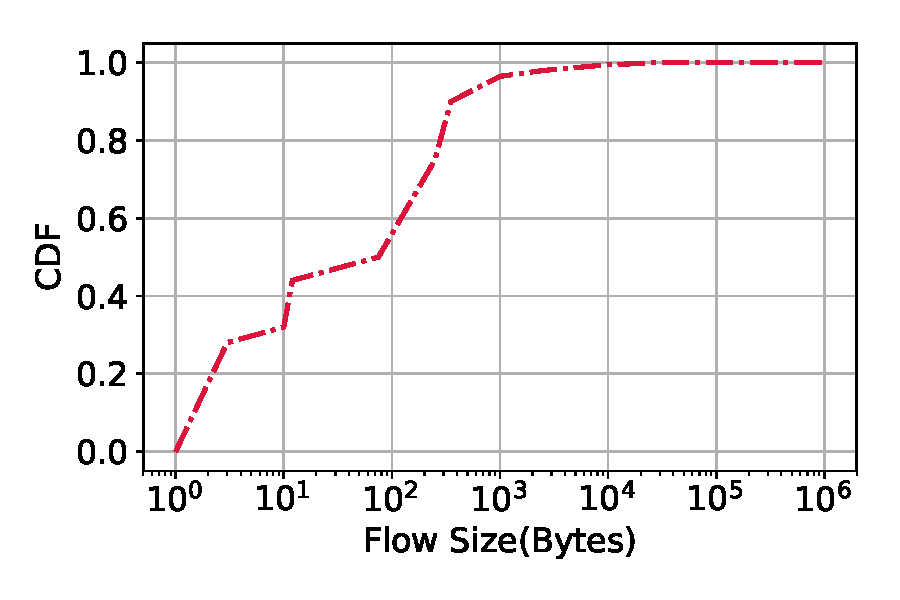
\includegraphics[width=3in]{pic/cdf.pdf}}
%\caption{Flow Size Distributions Used For Evaluation}
%\label{flow-size}
%\end{figure}

\begin{figure}[t]
\centering
\subfigure[Network topology]{\label{topo}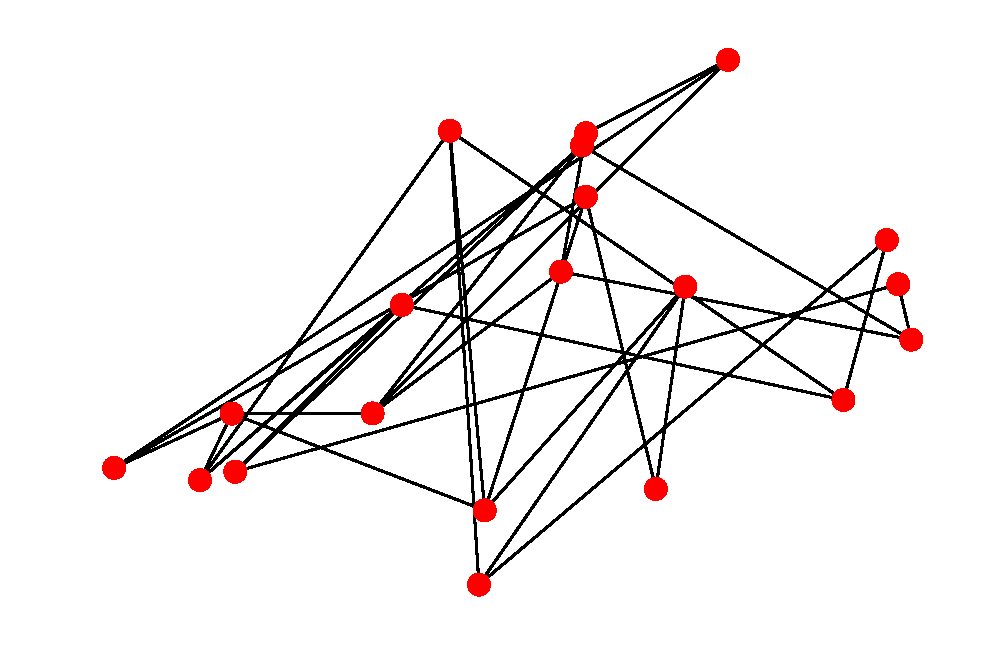
\includegraphics[width=1.7in]{pic/topo.pdf}}
\subfigure[Flow size distributions]{\label{flow-size}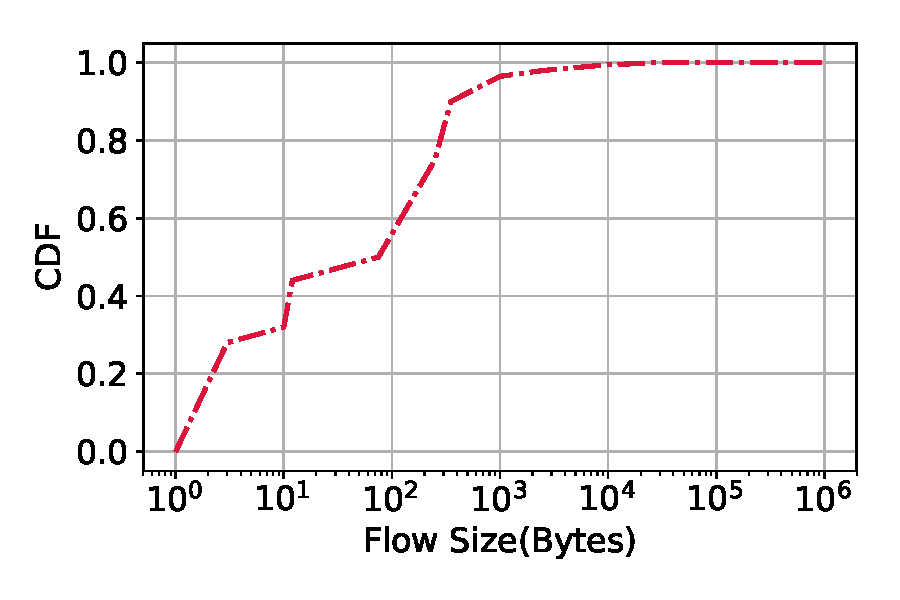
\includegraphics[width=1.7in]{pic/cdf.pdf}}
\caption{Network topology and Workload}
\label{topo-and-workload}
\end{figure}

%\begin{figure}[t]
%\centerline{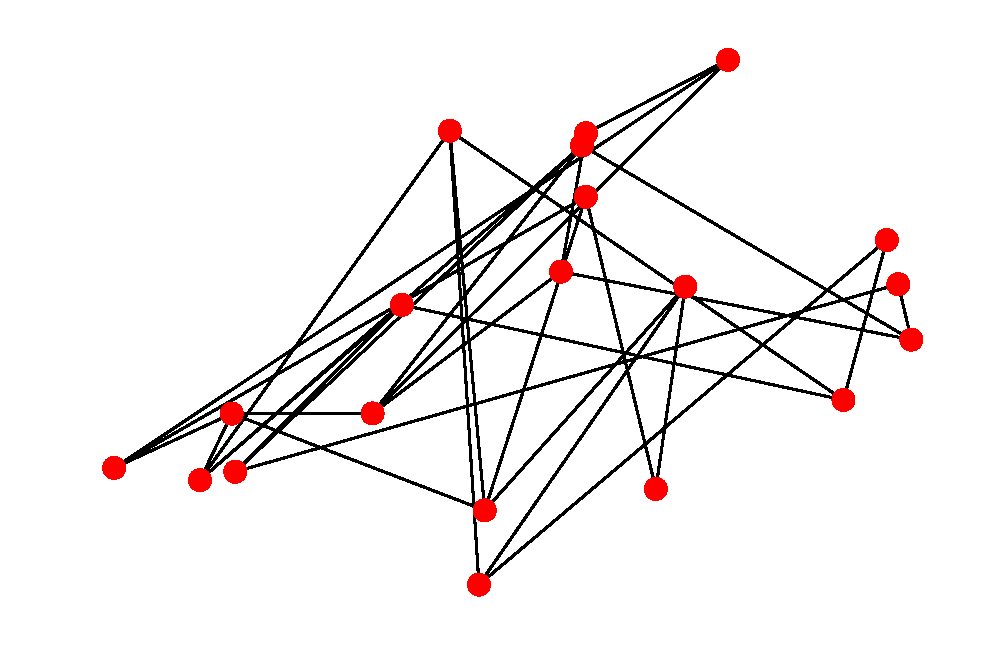
\includegraphics[width=3in]{pic/topo.pdf}}
%\caption{Network Topology}
%\label{topo}
%\end{figure}
%
%\begin{table}[t]
%\caption{Flow Size Distributions Used For Evaluation}
%\begin{center}
%\begin{tabular}{|c|c|c|c|c|c|c|c|}
%\hline
%\textbf{Size(bytes)}&{$10^0$}&{$10^1$}&{$10^2$} &{$10^3$} &{$10^4$} &{$10^5$} &{$10^6$} \\
%\hline
%\textbf{CDF}&{$0.28$}&{$0.32$}&{$0.58$} &{$0.965$} &{$0.995$} &{$0.9999$} &{$1$} \\
%\hline
%\end{tabular}
%\label{flow-size}
%\end{center}
%\end{table}

\emph{2) Metrics and compared methods}: Although the focus of DPRO is on the conventional optimization objective of minimizing link over-utilization (a.k.a. minimizing congestion) from traffic engineering literature, it can also influence the changes of other metrics such as flow completion time and packet delay to some extent. Therefore, we choose link max-link-utilization and flow completion time as well as packet delay as performance metrics to evaluate DPRO. Also, we compared our approach with three widely used baseline solutions:
%as well as a model while training: \cite{Chiesa2016Lying}\cite{Azar2003Optimal}\cite{Fortz2004Increasing}
\begin{itemize}
\item Shortest Path (SP): each source-destination pair uses the shortest path to deliver all its packets.
\item Equal Cost Multi-Path (ECMP): each source-destination pair evenly distributes its traffic load to $K$ candidate paths.
\item Dynamic Routing (LINEAR)\cite{Fortz2002}: it obtains TE solutions by modeling link loads and the cost (which is the same as link weights in DPRO) to a piecewise linear function. The cost of the link $l$ has to do with the relation between $l(a)$ and $c(a)$, as shown in function $\Phi_a$.
\end{itemize}

\begin{equation*}
\Phi_a(x)=\left\{
\begin{array}
{l}1\;\;\;\;\;\; \text{if}\;x\in\lbrack0,\frac13c(a)),
\\ 3\;\;\;\;\;\;\text{if}\;x\in\lbrack\frac13c(a),\frac23c(a)),
\\10\;\;\;\;\text{if}\;x\in\lbrack\frac23c(a),\frac56c(a)),
\\100\;\;\text{if}\;x\in\lbrack\frac56c(a),\infty).
\end{array}\right.
\end{equation*}
\subsection{Performance Results}\label{results}
To better understand experiments, only 2 edge nodes are selected to act as clients and 6 servers are chosen to reply to clients' requests. Each source node creates 6 TCP connections and sends the flow requests with flow sizes in polling. And each server replies with required flows to clients. Otherwise, we set the update period as 5 seconds and the sample period as 1 second, that is, $T_u=5s$ and $T_s=1s$. Each source-destination pair has two optimal paths, that is, $K=2$.

\emph{1) Online training results}: We show the performance of DPRO during the online learning procedure in terms of the reward. For illustration and comparison purposes, we normalize and smooth the reward values using a commonly-used method $(r-r_{min})/(r_{max}-r_{min})$ (where $r$ is the actual reward, $r_{min}$ and $r_{max}$ are the minimum and maximum rewards during online learning respectively) in Fig.\ref{reward-online}. Compared to ECMP, which we regard as a baseline, DPRO quickly (within just a couple of hundreds of decision epochs) reaches a good solution (that gives a high reward), while ECMP seems to have no awareness of traffic load and perform stable and low reward values in all the training epochs. As expected, we can see from Fig.\ref{reward-online} that DPRO significantly outperforms ECMP in terms of the max-link-utilization because its reward function is set to minimizing it.
\begin{figure}[t]
\centerline{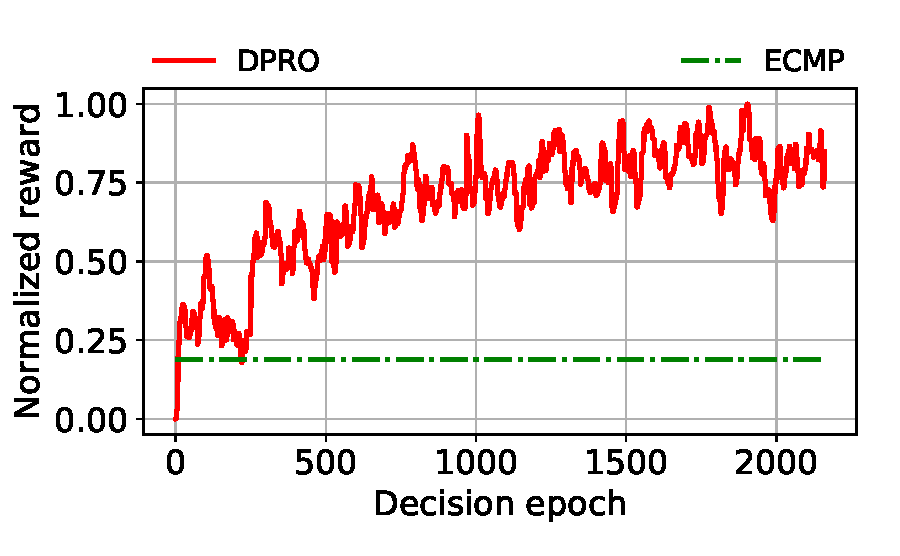
\includegraphics[width=3in]{pic/reward.pdf}}
\caption{Reward during online learning}
\label{reward-online}
\end{figure}

\emph{2) Performance of max-link-utilization}: To test the performance of all four methods subject to the max-link-utilization under different traffic loads, we set the traffic rate to 80Mbps initially and increase the traffic rate with a step size of 5 Mbps for each run. The traffic pattern is the same as the training period. Besides, we also add an evaluation under training traffic pattern with background traffic to illustrate the generality of DPRO. The background traffic is injected into our network at a rate of 200 packets per second through three edge nodes. We present the corresponding experiment results in Fig.\ref{reward-traffic}. Note that the numbers on the x-axis are the values of the corresponding traffic rate and the numbers on the y-axis are the max ratios between the link load and the link capacity of four TE methods.
%As expected, we can see from Fig.\ref{reward-traffic} that DPRO outperforms all the other methods in terms of the max-link-utilization because its reward function is set to minimizing it.
\begin{figure}[t]
\centering
\subfigure[Without background traffic]{\label{reward:a}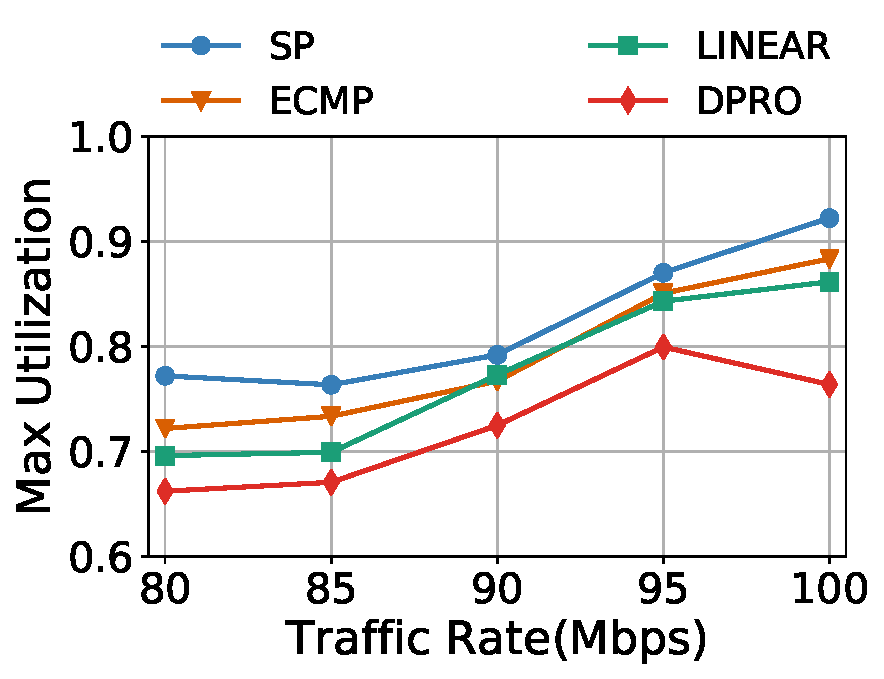
\includegraphics[width=1.7in]{pic/reward-without-back.pdf}}
\subfigure[With background traffic]{\label{reward:b}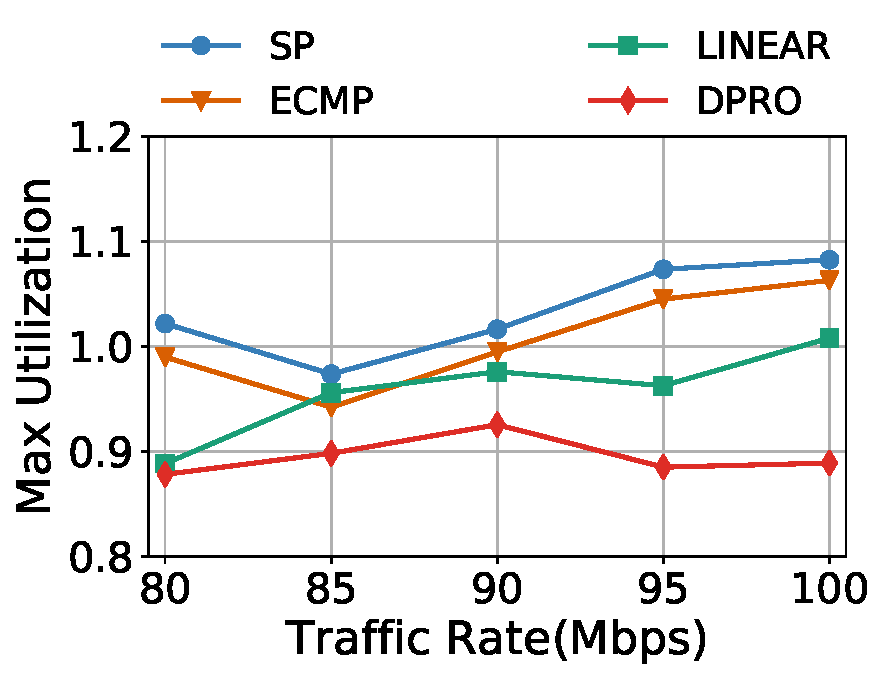
\includegraphics[width=1.7in]{pic/reward-with-back.pdf}}
\caption{Max utilization of all the methods over different traffic loads}
\label{reward-traffic}
\end{figure}

When the traffic load is without background traffic, as shown in Fig.\ref{reward:a}, DPRO always keeps the max-link-utilization below 0.8, while all the other three methods even up to 0.85 with the traffic load increases. Overall, DPRO achieves an average reduction of $13.9\%$, $9.3\%$ and $6.9\%$ respectively, compared to SP, ECMP, and LINEAR. When the traffic load is with background traffic, as shown in Fig.\ref{reward:b}, DPRO significantly maintains the max-link-utilization at about 0.9, with a floating range at 0.02. All the other three methods lead to poor performance with max-link-utilization up to 1.0, which can easily cause network congestion. On average, DPRO outperforms SP, ECMP, and LINEAR by $15.5\%$, $12.6\%$ and $7.1\%$ respectively.

\emph{3) Effective of FCT and packet delay}: Network congestion affects flow completion time and packet delay to some extent. Fig.\ref{performance} shows the FCT and packet delay under such a traffic pattern as the online learning procedure. By using DPRO, the average FCT (as shown in Fig.\ref{perfor-no-traffic:a}) is reduced by $11.4\%$, $6.1\%$ and $18.8\%$ compared with SP, ECMP, and LINEAR. And the 99th percentile FCT is cut down from $156.7ms$ to $140ms$, more than $19.2\%$ improvement that LINEAR. Note that as for packet delay (as shown in Fig.\ref{perfor-no-traffic:b}), these four TE approaches have similar delay performance. Especially, SP has the smallest average packet delay than the other three approaches. This is because that the training traffic load is quite light and the overall network link utilization is low, and only one single path is chosen to forward packets between a pair of nodes in SP while the other three methods have two, thus the advantages of multipath have no chances to show.
\begin{figure}[t]
\centering
\subfigure[FCT]{\label{perfor-no-traffic:a}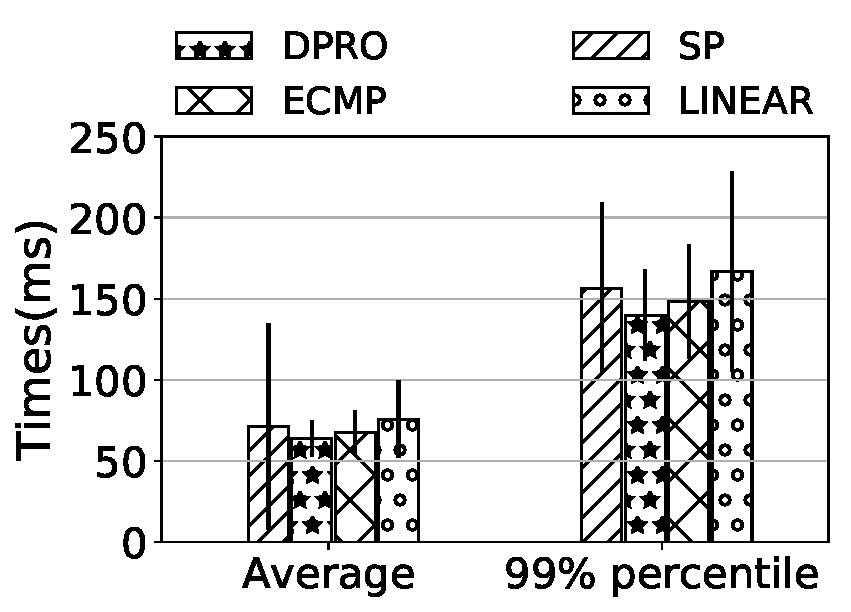
\includegraphics[width=1.7in]{pic/fct-1-2.pdf}}
\subfigure[Packet delay]{\label{perfor-no-traffic:b}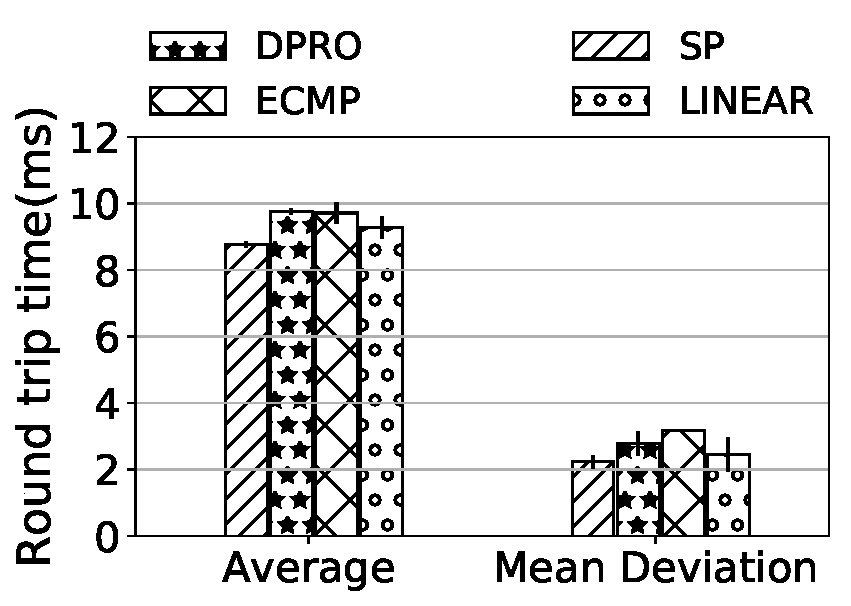
\includegraphics[width=1.7in]{pic/packet-delay-1-2.pdf}}
\caption{FCT and packet delay without background traffic}
\label{performance}
\end{figure}

Fig.\ref{performance-with-bgf} shows the FCT and packet delay respectively under training traffic patterns with background traffic. DPRO has much better performance than the other three methods because it can adjust routing strategy at the basis of network load status monitoring in real-time. Compared with SP, as shown in Fig.\ref{perfor-traffic:a}, DPRO reduces the average FCT by $7.2\%$ and the 99th percentile FCT by $7.1\%$. Especially, in terms of packet delay, as shown in Fig.\ref{perfor-traffic:b}, DPRO outperforms SP, ECMP, and LINEAR by $56.8\%$, $27.2\%$, and $75.3\%$ respectively in mean deviation, and $24.8\%$, $17.1\%$, and $53.8\%$ in average packet delay.
\begin{figure}[t]
\centering
\subfigure[FCT]{\label{perfor-traffic:a}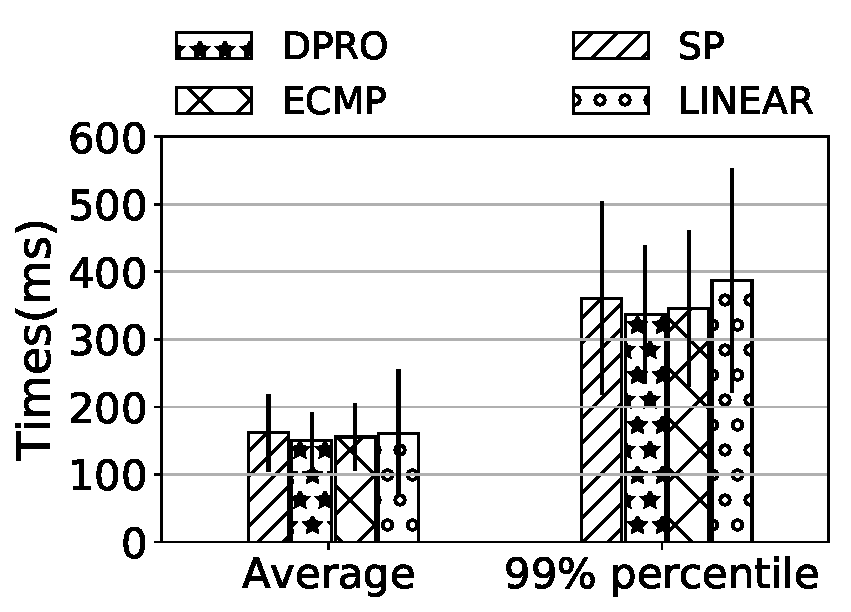
\includegraphics[width=1.7in]{pic/fct-with-bgf-1-2.pdf}}
\subfigure[Packet delay]{\label{perfor-traffic:b}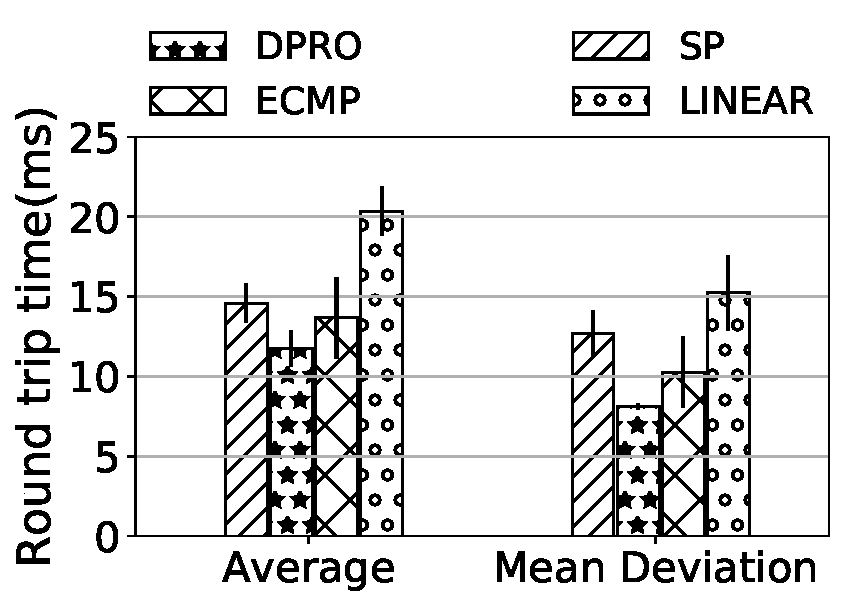
\includegraphics[width=1.7in]{pic/packet-delay-with-bgf-1-2.pdf}}
\caption{FCT and packet delay with background traffic}
\label{performance-with-bgf}
\end{figure}

\emph{4) Measurement overhead}: The measurement overhead via INT in our approach is very low, especially on network bandwidth. In our proposal, we set the size of one int\_header is 24 bit and the maximum hops of one route is 8. Thus, the maximum size of measurement information carried by a sampling packet is 24 bytes.

From the view of the only packet, the Ethernet header is 18 bytes, and the IP header, as well as TCP header, is generally 20 bytes. Thus, the largest proportion of int\_headers in the headers of one packet is $24/(24+18+20*2)=29.3\%$. As we know, the maximum length of Ethernet packet is 1518 bytes and the minimum length is 64 bytes, therefore, we can calculate that the largest proportion of measurement information is $24/(24+64)=27.3\%$ in minimum Ethernet packet and $24/(24+1518)=1.56\%$ in maximum Ethernet packet.

From the perspective of bandwidth resources, DPRO has an extra-low requirement to bandwidth resources. As illustrated before, the sampling period is set to 1 second and only 14 edge switches are responsible for taking sampling tasks (based on the simulation topology). Therefore, the bandwidth occupied by network measurement is $3Bps *14=42Bps$, which is only 0.000336\% of the link capacity (the link capacity is set to 100MBps).

\section{Conclusion}
In this paper, we investigated the traffic engineering problem in SDN, for which we aimed to find the policy that minimizes network congestion with network load status changes. We explored in-band network telemetry technology based on programmable language P4 to measure network load status with ultra-low overhead. We introduced a reinforcement learning PPO algorithm to the controller to solve the problem that the relationship between network load status and routing strategies is hard to model and calculate. We named our approach DPRO. Evaluation results showed that DPRO offers significant performance improvement compared to three baseline TE solutions concerning three metrics including max-link-utilization, flow completion time, and packet delay.

\bibliographystyle{IEEEtran}
\bibliography{mylib}
\vspace{12pt}
%\color{red}
%contain guidance text for composing and formatting conference papers. Please ensure that all template text is removed from your conference paper before submission to the conference. Failure to remove the template text from your paper may result in your paper not being published.
\end{document}
